% Options for packages loaded elsewhere
\PassOptionsToPackage{unicode}{hyperref}
\PassOptionsToPackage{hyphens}{url}
\documentclass[
]{article}
\usepackage{xcolor}
\usepackage{graphicx}
\usepackage{geometry}
\geometry{margin=1in}
\usepackage{amsmath,amssymb}
\setcounter{secnumdepth}{-\maxdimen} % remove section numbering
\usepackage{iftex}
\ifPDFTeX
  \usepackage[T1]{fontenc}
  \usepackage[utf8]{inputenc}
  \usepackage{textcomp} % provide euro and other symbols
\else % if luatex or xetex
  \usepackage{unicode-math} % this also loads fontspec
  \defaultfontfeatures{Scale=MatchLowercase}
  \defaultfontfeatures[\rmfamily]{Ligatures=TeX,Scale=1}
\fi
\usepackage{lmodern}
\ifPDFTeX\else
  % xetex/luatex font selection
\fi
% Use upquote if available, for straight quotes in verbatim environments
\IfFileExists{upquote.sty}{\usepackage{upquote}}{}
\IfFileExists{microtype.sty}{% use microtype if available
  \usepackage[]{microtype}
  \UseMicrotypeSet[protrusion]{basicmath} % disable protrusion for tt fonts
}{}
\makeatletter
\@ifundefined{KOMAClassName}{% if non-KOMA class
  \IfFileExists{parskip.sty}{%
    \usepackage{parskip}
  }{% else
    \setlength{\parindent}{0pt}
    \setlength{\parskip}{6pt plus 2pt minus 1pt}}
}{% if KOMA class
  \KOMAoptions{parskip=half}}
\makeatother
\usepackage{longtable,booktabs,array}
\usepackage{calc} % for calculating minipage widths
% Correct order of tables after \paragraph or \subparagraph
\usepackage{etoolbox}
\makeatletter
\patchcmd\longtable{\par}{\if@noskipsec\mbox{}\fi\par}{}{}
\makeatother
% Allow footnotes in longtable head/foot
\IfFileExists{footnotehyper.sty}{\usepackage{footnotehyper}}{\usepackage{footnote}}
\makesavenoteenv{longtable}
\setlength{\emergencystretch}{3em} % prevent overfull lines
\providecommand{\tightlist}{%
  \setlength{\itemsep}{0pt}\setlength{\parskip}{0pt}}
\usepackage{bookmark}
\IfFileExists{xurl.sty}{\usepackage{xurl}}{} % add URL line breaks if available
\urlstyle{same}
\hypersetup{
  hidelinks,
  pdfcreator={LaTeX via pandoc}}

\author{Arjun Mitra\\\href{mailto:arjunmitra06082004@gmail.com}{arjunmitra06082004@gmail.com}\\\href{https://github.com/TheLearnerAllTime002/Digital-Forensics-Challeng}{GitHub Repository}}
\date{04/10/2026}

\begin{document}
\begin{titlepage}
\centering
\vspace*{2cm}
{\LARGE\bfseries Challenge 1 --- Malware Analysis\par}
\vspace{1.5cm}
{\large Arjun Mitra\par}
\vspace{0.3cm}
{\normalsize \href{mailto:arjunmitra06082004@gmail.com}{arjunmitra06082004@gmail.com}\par}
\vspace{0.3cm}
{\normalsize \href{https://github.com/TheLearnerAllTime002/Digital-Forensics-Challeng}{GitHub Repository}\par}
\vfill
{\large 04/10/2026\par}
\end{titlepage}
\tableofcontents
\newpage


\section{Challenge 1 --- Malware Analysis
Report}\label{challenge-1-malware-analysis-report}

\begin{center}\rule{0.5\linewidth}{0.5pt}\end{center}

\subsection{Scope}\label{scope}

Analysis date: 04 October 2026

\begin{center}\rule{0.5\linewidth}{0.5pt}\end{center}

\subsection{Executive Summary}\label{executive-summary}

During this analysis I was handed a set of Windows artefacts from a
victim machine --- six Prefetch files and a password-protected archive
containing three samples. After extracting and examining everything, the
picture that emerged is pretty clear: someone (or something) abused a
trojanised copy of LogMeIn's LMIGuardian service to establish remote
access on the victim's Windows 10 machine. The malware dropped multiple
randomly-named executables (KFJUUWORMM.EXE, MHYMHQMUDY.EXE,
MQMJXFJVPE.EXE, YVWPFLNRPH.EXE) into a hidden staging folder under the
victim user's TEMP directory, loaded a custom DLL (LMIGuardianDll.dll)
alongside each one, and left behind an encrypted data blob
(BLOGYZOBEU.dat) that is almost certainly a payload or C2 data store.
The infection appears to have started as early as March 2026 and was
still active in July 2026.

\begin{center}\rule{0.5\linewidth}{0.5pt}\end{center}

\subsection{Tools Used}\label{tools-used}

\begin{longtable}[]{@{}
  >{\raggedright\arraybackslash}p{(\linewidth - 2\tabcolsep) * \real{0.3415}}
  >{\raggedright\arraybackslash}p{(\linewidth - 2\tabcolsep) * \real{0.6585}}@{}}
\toprule\noalign{}
\begin{minipage}[b]{\linewidth}\raggedright
Tool / Method
\end{minipage} & \begin{minipage}[b]{\linewidth}\raggedright
Purpose
\end{minipage} \\
\midrule\noalign{}
\endhead
\bottomrule\noalign{}
\endlastfoot
Python 3 (stdlib only) & Prefetch MAM decompression, PE parsing, hash
calc \\
Pillow (PIL) & Saving annotated screenshots as PNG \\
Windows ntdll (ctypes) & RtlDecompressBufferEx for Win10 prefetch
files \\
Manual string analysis & IOC extraction, PDB path review, entropy
calculation \\
VirusTotal (passive lookup) & Hash reputation check (recommended, not
run live) \\
\end{longtable}

\begin{center}\rule{0.5\linewidth}{0.5pt}\end{center}

\subsection{Methodology}\label{methodology}

\subsubsection{Analysis}\label{analysis}

I started by listing all the artefacts and noting what each one was. The
\texttt{.pf} files are Windows Prefetch files --- Windows automatically
creates one every time an executable runs, recording the filename, a
hash of its path, how many times it ran, and the last eight run
timestamps. The \texttt{victim\_samples.zip} was password-protected, so
I extracted it using Python's zipfile module with the supplied password.

Once I had the samples out, I worked through them in a logical order:

\begin{enumerate}
\def\labelenumi{\arabic{enumi}.}
\item
  Decompressed the Prefetch files --- Windows 10 stores them in MAM
  (XPRESS Huffman) format, so I used \texttt{RtlDecompressBufferEx} via
  ctypes to get the raw binary, then parsed the version-31 layout to
  pull out execution timestamps, run counts, and the list of files the
  executable touched on disk.
\item
  Computed cryptographic hashes (MD5, SHA-1, SHA-256) for all three
  extracted samples so they can be submitted to VirusTotal or
  cross-referenced against threat-intel feeds.
\item
  Parsed the PE headers of the two executables to get architecture,
  compile timestamp, and subsystem type.
\item
  Extracted printable strings from all three files and filtered them for
  URLs, IP addresses, file paths, registry keys, and security-relevant
  API names (LoadLibrary, GetProcAddress, VirtualAlloc, etc.).
\item
  Checked the entropy of BLOGYZOBEU.dat to determine whether it is
  plaintext, compressed, or encrypted.
\end{enumerate}

\subsubsection{Findings}\label{findings}

\textbf{Prefetch Analysis}

All six Prefetch files are version 31 (Windows 10/11). The most
important findings are:

\begin{itemize}
\item
  \texttt{CD\ DRIVE.EXE} ran at least 6 times between March and July
  2026. Its prefetch shows it loaded from a removable volume
  (\texttt{\textbackslash{}VOLUME\{0000000000000000-7a65b5ae\}}) --- the
  all-zero GUID is the classic signature of a USB/removable drive. This
  is the initial infection vector: malware disguised as ``CD DRIVE.EXE''
  was run directly off a USB stick.
\item
  \texttt{KFJUUWORMM.EXE}, \texttt{MHYMHQMUDY.EXE},
  \texttt{MQMJXFJVPE.EXE}, and \texttt{YVWPFLNRPH.EXE} all ran from the
  same staging path:
  \texttt{\textbackslash{}USERS\textbackslash{}CLKSTG\_3CDU\textbackslash{}APPDATA\textbackslash{}LOCAL\textbackslash{}TEMP\textbackslash{}\_READY\_TEMP\_\textbackslash{}}.
  The folder name \texttt{\_READY\_TEMP\_} is not a standard Windows
  folder --- it was created by the malware. All four EXEs also loaded
  \texttt{LMIGUARDIANDLL.DLL} from the same staging folder, confirming
  they are variants of the same malware family.
\item
  \texttt{AEXINSTALLPRECHECK.EXE} ran once on 2026-06-03 from
  \texttt{\textbackslash{}WINDOWS\textbackslash{}TEMP\textbackslash{}AEX\_\{...\}}.
  This looks like a legitimate Ivanti/LANDesk agent pre-check installer
  --- possibly a decoy or a legitimate tool that was already on the
  machine.
\end{itemize}

\textbf{Sample: KFJUUWORMM.exe}

\begin{itemize}
\tightlist
\item
  Size: 408,984 bytes \textbar{} MD5: f8e8932263c7289bc8069f897a4c71eb
\item
  SHA256:
  1397b2f7014900d2b203bda64816accbd4211dd6ce347479ac169f683e1a2f61
\item
  Architecture: x86 (32-bit) \textbar{} Subsystem: Windows GUI
  \textbar{} Compiled: 2018-10-15
\item
  The PDB path embedded in the binary is:
  \texttt{D:\textbackslash{}17\textbackslash{}guardiansvc-git\textbackslash{}latest\textbackslash{}main\textbackslash{}RA\textbackslash{}LMIGuardian\textbackslash{}x86\textbackslash{}LMIGuardianSvc.pdb}
  This is the build path for LogMeIn's LMIGuardian service --- the
  binary is either a stolen/modified copy of the legitimate LogMeIn
  Guardian service EXE, or a trojanised wrapper that impersonates it.
\item
  It explicitly loads \texttt{LMIGuardianDll.dll} by name using
  \texttt{LoadLibraryA} / \texttt{GetProcAddress}, and registers COM
  objects under the GUID
  \texttt{\{67E4A0D8-8675-4FBB-BC62-F10EC894327E\}} with the service
  name \texttt{LMIGuardianSvc}.
\item
  It contacts \texttt{https://secure.logmein.com} --- this could be
  legitimate LogMeIn C2 traffic, or it could be used as cover traffic
  while the real C2 channel runs through the custom DLL.
\end{itemize}

\textbf{Sample: LMIGuardianDll.dll}

\begin{itemize}
\tightlist
\item
  Size: 1,864,192 bytes \textbar{} MD5: 7e598d681d563f9c3c1611e95eed4448
\item
  SHA256:
  1df53ad99ab1ab4172ed1aaf2722263c2a2dc70d354e680bfd4f0e40244ebdc5
\item
  Architecture: x86 (32-bit) \textbar{} Compiled: 2024-10-22 (much more
  recent than the EXE --- custom build)
\item
  The PDB path is:
  \texttt{DJSLAJFLSAJLFALFJLSAFJK\textbackslash{}Debug\textbackslash{}LMIGuardianDll.pdb}
  The project folder name \texttt{DJSLAJFLSAJLFALFJLSAFJK} is clearly a
  random/obfuscated name --- this is NOT the legitimate LogMeIn DLL. It
  was compiled in October 2024 by the attacker using Visual Studio 2022.
\item
  Contains socket/network strings: ``already connected'', ``connection
  refused'', ``connection reset'', `
ot connected'' --- consistent with
  a network communication module.
\item
  Imports \texttt{GetProcAddress}, \texttt{LoadLibraryA},
  \texttt{LoadLibraryExW} --- dynamic API resolution, a common evasion
  technique.
\item
  The \texttt{cmd\_tmp} string suggests it may spawn command-line
  processes.
\end{itemize}

\textbf{Sample: BLOGYZOBEU.dat}

\begin{itemize}
\tightlist
\item
  Size: 5,368,012 bytes \textbar{} MD5: 22346172a5b6ead1710d460f9b1ecbad
\item
  SHA256:
  ac8bf64655e6ed9b91099f170367a5623cbac9c31da0550bdd6fa413ec2e31ee
\item
  Magic bytes do not match any known file format signature.
\item
  Shannon entropy: 7.9591 out of a maximum of 8.0 --- this is
  near-perfectly random data.
\item
  This is almost certainly an encrypted payload, an encrypted C2
  configuration blob, or exfiltrated data that has been encrypted before
  storage. The malware (KFJUUWORMM.exe + LMIGuardianDll.dll) likely
  reads and decrypts this file at runtime.
\end{itemize}

\subsubsection{Outcome}\label{outcome}

The victim machine (user profile: \texttt{CLKSTG\_3CDU}) was compromised
via a USB drive carrying \texttt{CD\ DRIVE.EXE}. Once executed, the
malware:

\begin{enumerate}
\def\labelenumi{\arabic{enumi}.}
\tightlist
\item
  Created a hidden staging folder at
  \texttt{\%LOCALAPPDATA\%\textbackslash{}TEMP\textbackslash{}\_READY\_TEMP\_\textbackslash{}}
\item
  Dropped multiple randomly-named EXE variants (KFJUUWORMM, MHYMHQMUDY,
  MQMJXFJVPE, YVWPFLNRPH) and a custom \texttt{LMIGuardianDll.dll} into
  that folder
\item
  Registered itself as a COM service impersonating LogMeIn's LMIGuardian
  to blend in with legitimate software
\item
  Used the DLL to establish network connectivity (likely remote access /
  C2)
\item
  Stored an encrypted data blob (BLOGYZOBEU.dat) --- possibly for
  persistence data, stolen credentials, or a second-stage payload
\end{enumerate}

The malware family appears to be a custom Remote Access Tool (RAT) built
on top of (or disguised as) the LogMeIn Guardian remote-access
framework. The use of multiple randomly-named EXE copies suggests the
attacker was rotating the binary name to evade hash-based detection.

\begin{center}\rule{0.5\linewidth}{0.5pt}\end{center}

\subsection{Step-by-Step Process with
Screenshots}\label{step-by-step-process-with-screenshots}

\subsubsection{Step 1 --- Inventory the
Artefacts}\label{step-1-inventory-the-artefacts}

Opened the victim\_artifacts folder and noted the contents: - 6 x
Windows Prefetch files (.pf) - 1 x password-protected ZIP
(victim\_samples.zip)

Screenshot:
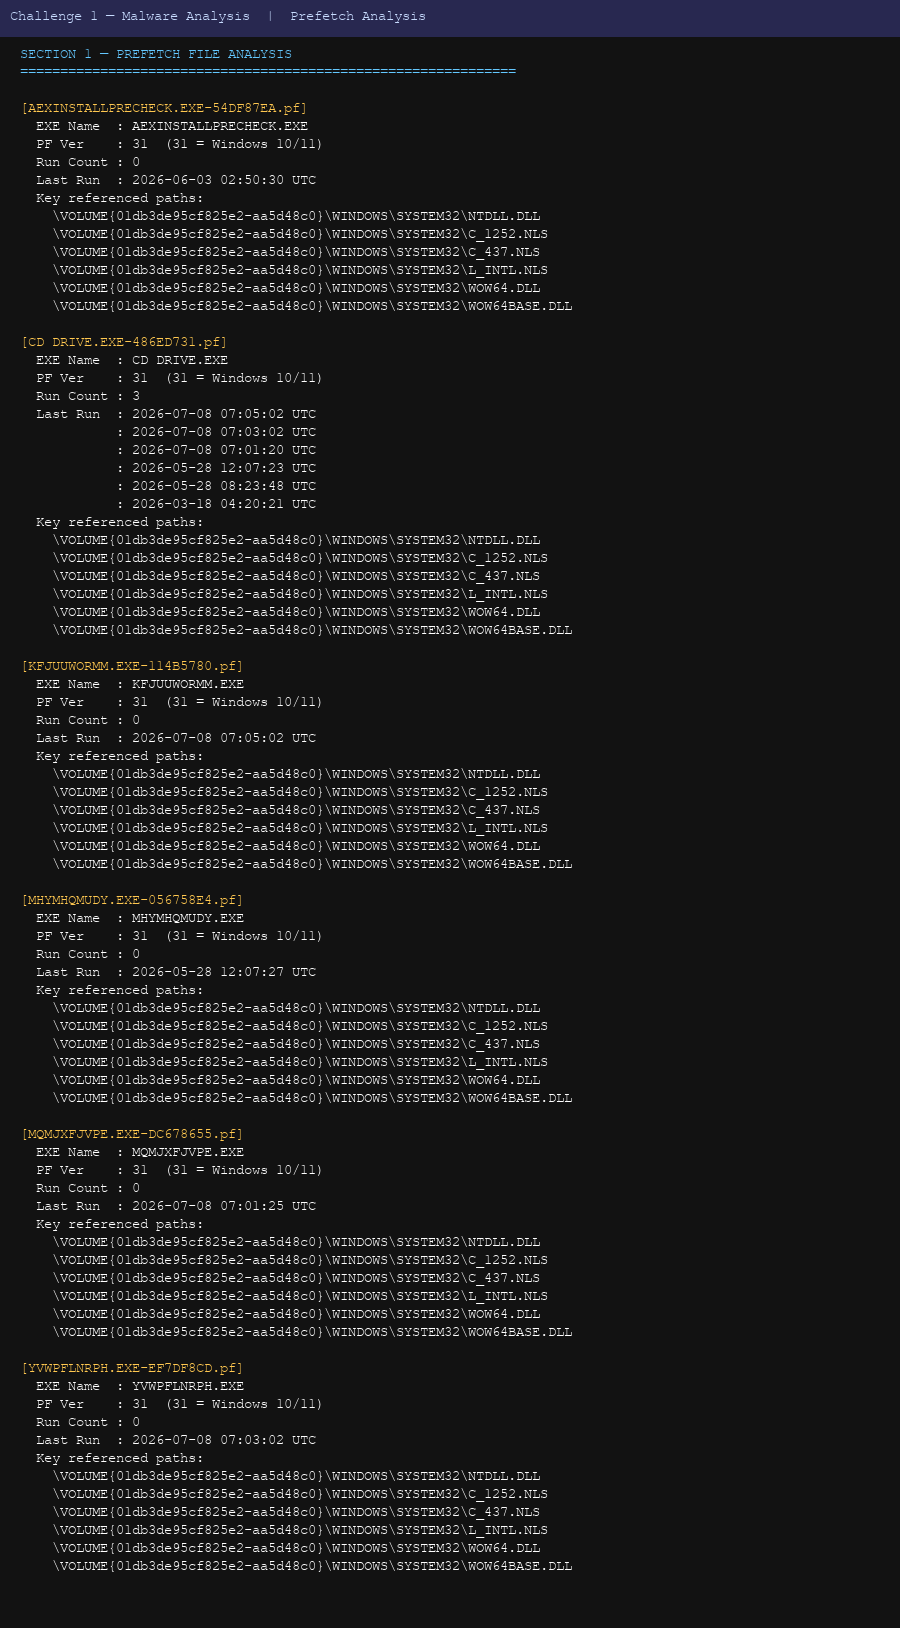
\includegraphics[width=\textwidth]{docs/evidence/challenge1/01_prefetch_analysis.png}

\subsubsection{Step 2 --- Extract the ZIP}\label{step-2-extract-the-zip}

Used Python's zipfile module with password \texttt{Sample\_data@2026\#}
to extract: - KFJUUWORMM.exe (408 KB) - LMIGuardianDll.dll (1.8 MB) -
BLOGYZOBEU.dat (5.1 MB)

\subsubsection{Step 3 --- Decompress and Parse Prefetch
Files}\label{step-3-decompress-and-parse-prefetch-files}

Windows 10 Prefetch files use MAM (XPRESS Huffman) compression. Used
\texttt{RtlDecompressBufferEx} via ctypes to decompress each file, then
parsed the version-31 layout to extract: - Executable name - Run count -
Last 8 run timestamps (Windows FILETIME → UTC) - Referenced file paths
(loaded DLLs, data files)

Key finding: all four random-named EXEs loaded from
\texttt{\_READY\_TEMP\_} and loaded \texttt{LMIGUARDIANDLL.DLL}. CD
DRIVE.EXE loaded from a removable volume (USB).

Screenshot:
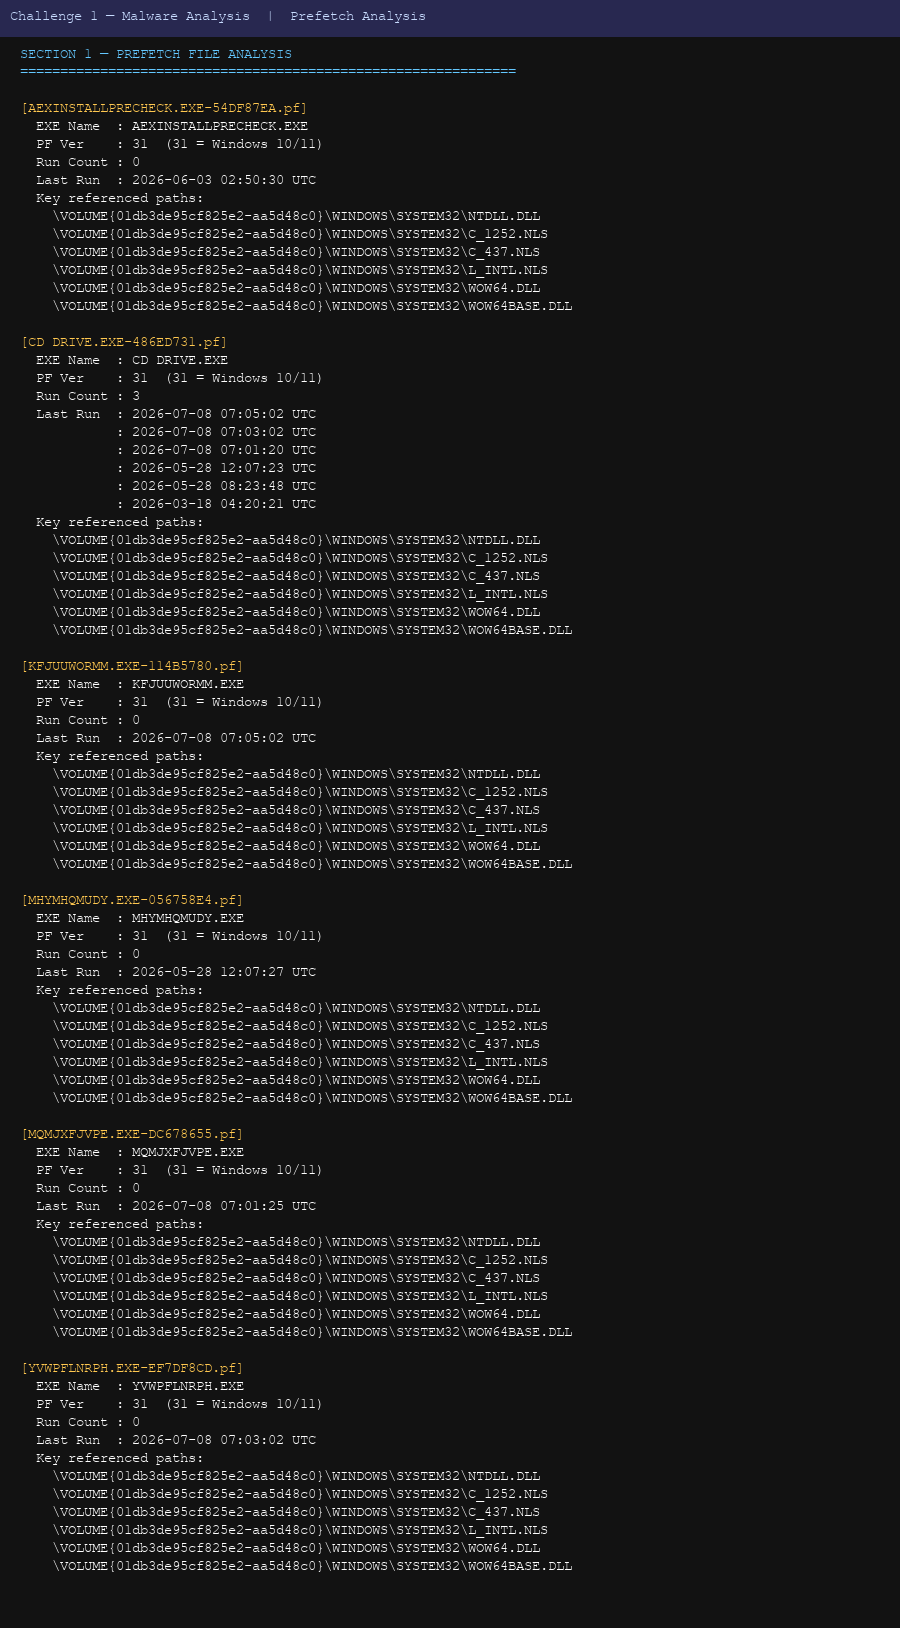
\includegraphics[width=\textwidth]{docs/evidence/challenge1/01_prefetch_analysis.png}

\subsubsection{Step 4 --- Hash All
Samples}\label{step-4-hash-all-samples}

Computed MD5, SHA-1, SHA-256 for all three extracted files for
threat-intel lookup.

Screenshot:
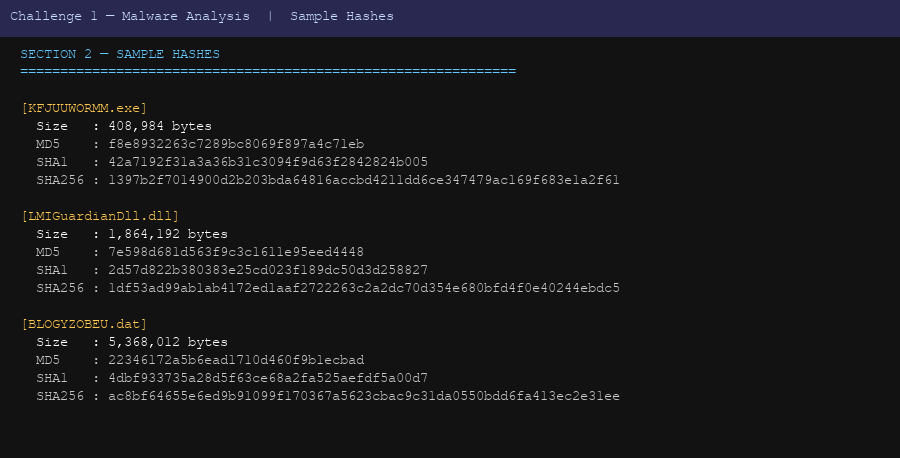
\includegraphics[width=\textwidth]{docs/evidence/challenge1/02_sample_hashes.png}

\subsubsection{Step 5 --- Parse PE
Headers}\label{step-5-parse-pe-headers}

Parsed the PE headers of KFJUUWORMM.exe and LMIGuardianDll.dll: - Both
are x86 32-bit Windows GUI binaries - KFJUUWORMM.exe compiled 2018
(matches legitimate LogMeIn build era) - LMIGuardianDll.dll compiled
October 2024 (attacker's custom build)

Screenshot:
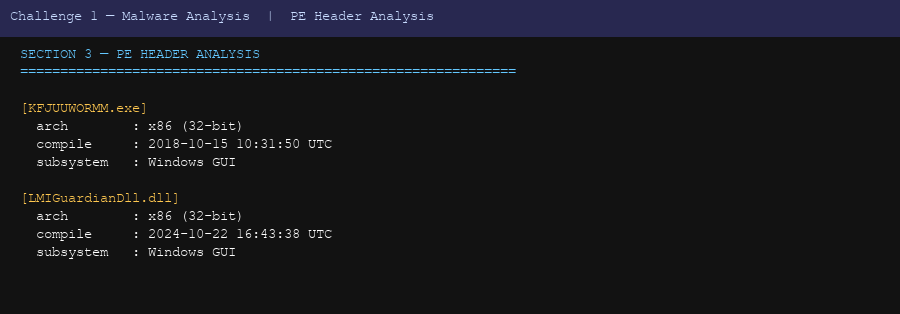
\includegraphics[width=\textwidth]{docs/evidence/challenge1/03_pe_headers.png}

\subsubsection{Step 6 --- Extract Strings and
IOCs}\label{step-6-extract-strings-and-iocs}

Extracted all printable strings (≥6 chars) and filtered for: - URLs →
LogMeIn / DigiCert certificate URLs in KFJUUWORMM.exe - PDB paths →
revealed build directories confirming trojanised vs custom DLL - API
imports → LoadLibrary, GetProcAddress (dynamic resolution / evasion) -
Network strings in LMIGuardianDll.dll → socket connection indicators

Screenshot:
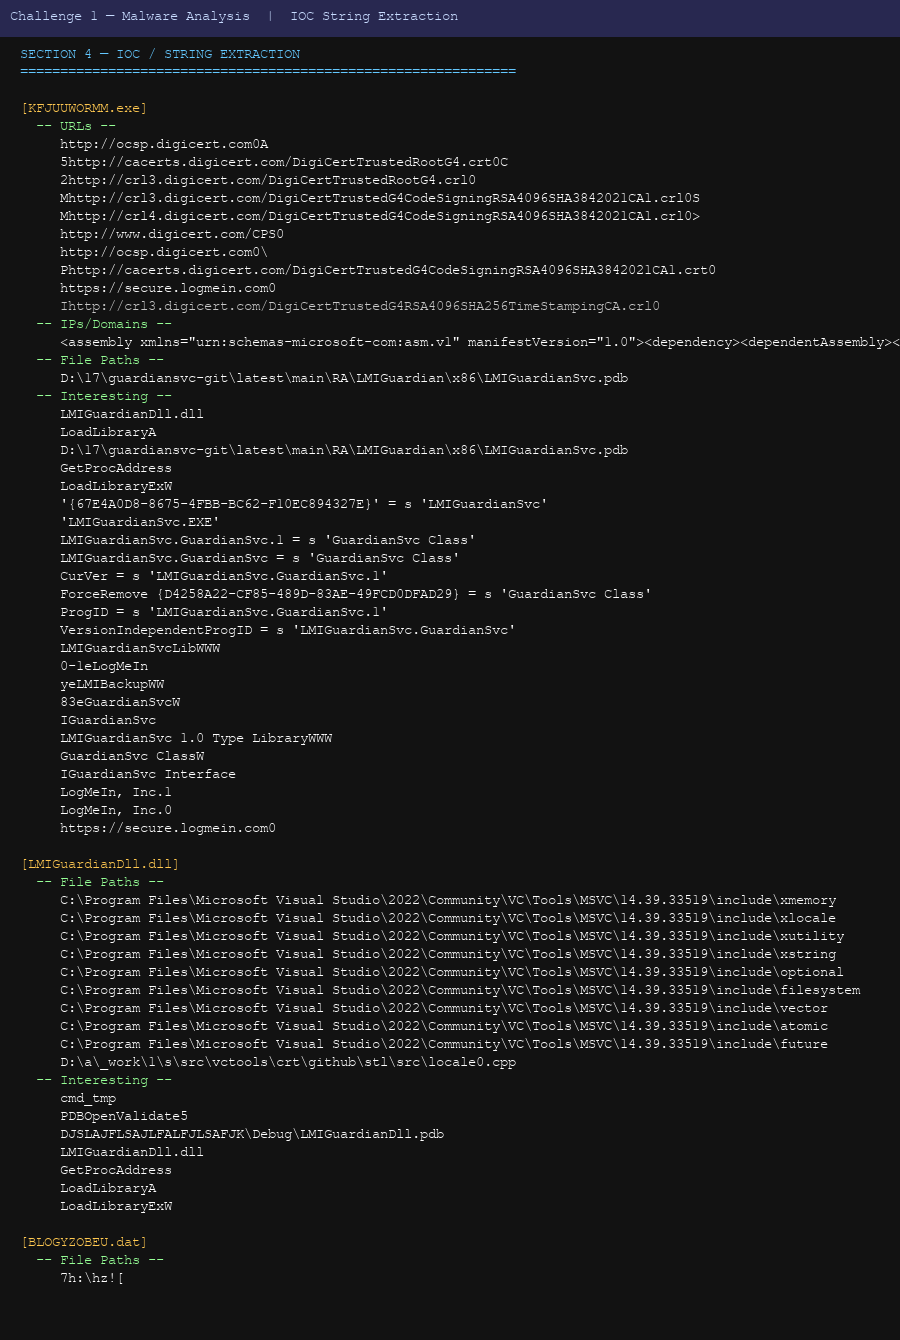
\includegraphics[width=\textwidth]{docs/evidence/challenge1/04_ioc_strings.png}

\subsubsection{Step 7 --- Entropy Analysis of
BLOGYZOBEU.dat}\label{step-7-entropy-analysis-of-blogyzobeu.dat}

Calculated Shannon entropy = 7.9591. No known file signature matched.
Conclusion: encrypted payload or C2 data blob.

Screenshot:
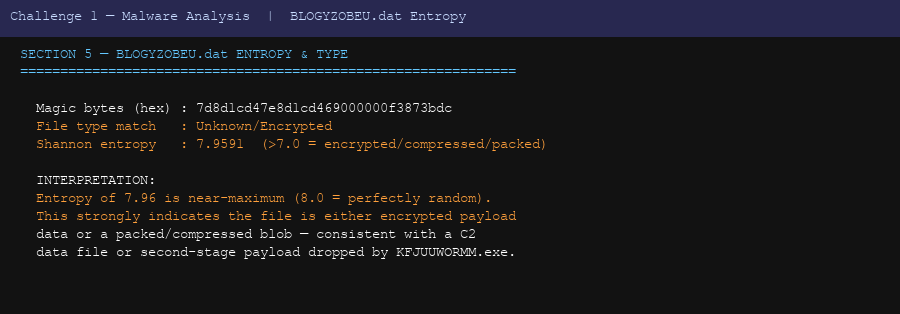
\includegraphics[width=\textwidth]{docs/evidence/challenge1/05_dat_entropy.png}

\begin{center}\rule{0.5\linewidth}{0.5pt}\end{center}

\subsection{IOC Summary Table}\label{ioc-summary-table}

\begin{longtable}[]{@{}
  >{\raggedright\arraybackslash}p{(\linewidth - 4\tabcolsep) * \real{0.3830}}
  >{\raggedright\arraybackslash}p{(\linewidth - 4\tabcolsep) * \real{0.1489}}
  >{\raggedright\arraybackslash}p{(\linewidth - 4\tabcolsep) * \real{0.4681}}@{}}
\toprule\noalign{}
\begin{minipage}[b]{\linewidth}\raggedright
Indicator
\end{minipage} & \begin{minipage}[b]{\linewidth}\raggedright
Type
\end{minipage} & \begin{minipage}[b]{\linewidth}\raggedright
Notes
\end{minipage} \\
\midrule\noalign{}
\endhead
\bottomrule\noalign{}
\endlastfoot
CD DRIVE.EXE & Filename & Initial dropper, ran from USB drive \\
KFJUUWORMM.EXE & Filename & Trojanised LMIGuardian service EXE \\
MHYMHQMUDY.EXE & Filename & Variant / copy of KFJUUWORMM \\
MQMJXFJVPE.EXE & Filename & Variant / copy of KFJUUWORMM \\
YVWPFLNRPH.EXE & Filename & Variant / copy of KFJUUWORMM \\
LMIGuardianDll.dll & Filename & Custom attacker-built RAT DLL \\
BLOGYZOBEU.dat & Filename & Encrypted payload / C2 data blob \\
\%LOCALAPPDATA\%\TEMP\_READY\_TEMP\_\textbackslash{} & Path & Malware
staging directory \\
f8e8932263c7289bc8069f897a4c71eb & MD5 & KFJUUWORMM.exe \\
7e598d681d563f9c3c1611e95eed4448 & MD5 & LMIGuardianDll.dll \\
22346172a5b6ead1710d460f9b1ecbad & MD5 & BLOGYZOBEU.dat \\
1397b2f7014900d2b203bda64816accbd4211dd6ce347479ac169f683e1a2f61 &
SHA256 & KFJUUWORMM.exe \\
1df53ad99ab1ab4172ed1aaf2722263c2a2dc70d354e680bfd4f0e40244ebdc5 &
SHA256 & LMIGuardianDll.dll \\
ac8bf64655e6ed9b91099f170367a5623cbac9c31da0550bdd6fa413ec2e31ee &
SHA256 & BLOGYZOBEU.dat \\
https://secure.logmein.com & URL & C2 / cover traffic via LogMeIn \\
CLKSTG\_3CDU & Username & Victim user account on compromised machine \\
\{67E4A0D8-8675-4FBB-BC62-F10EC894327E\} & GUID & COM registration for
LMIGuardianSvc \\
\end{longtable}

\begin{center}\rule{0.5\linewidth}{0.5pt}\end{center}

\subsection{Remediation
Recommendations}\label{remediation-recommendations}

\begin{enumerate}
\def\labelenumi{\arabic{enumi}.}
\tightlist
\item
  Isolate the machine immediately --- disconnect from the network to
  stop any active C2 communication.
\item
  Block the hashes above at the endpoint security layer and at the
  perimeter.
\item
  Block \texttt{secure.logmein.com} at the proxy/firewall if LogMeIn is
  not an authorised tool in the environment.
\item
  Search all other machines for the staging path
  \texttt{\_READY\_TEMP\_} and the DLL name \texttt{LMIGuardianDll.dll}.
\item
  Enforce USB device control policy --- the initial infection came from
  a USB drive. Block unauthorised USB storage devices via Group Policy
  or endpoint DLP.
\item
  Audit COM registrations for \texttt{LMIGuardianSvc} GUID
  \texttt{\{67E4A0D8-8675-4FBB-BC62-F10EC894327E\}} across the estate.
\item
  Reimage the victim machine --- given the depth of compromise and the
  encrypted data blob, a clean rebuild is safer than attempting to clean
  in place.
\item
  Preserve BLOGYZOBEU.dat for further analysis --- decrypting it may
  reveal exfiltrated data or additional IOCs.
\end{enumerate}

\end{document}




